\documentclass[a4paper,twoside,10pt,french]{scrartcl}
\usepackage[T1]{fontenc}
\usepackage{titlesec}
\usepackage{ulem}
\usepackage[dvipsnames]{xcolor}
\usepackage{color}
\usepackage{babel}
\usepackage{helvet}
\usepackage[utf8]{inputenc}
\usepackage[T1]{fontenc}
\usepackage{geometry}
\usepackage{graphicx}
\title{28 page 284 - C7}
\date{}
 \renewcommand*\familydefault{\sfdefault}
\geometry{a4paper}
% -------------------------------------------------------------------------------------------------
% ----------- Création des commandes de couleur pour les titres ----------
% -------------------------------------------------------------------------------------------------
\newcommand{\sectionred}[1]{{\color{red}{\uuline{\color{black}#1}}}}
\newcommand{\sectiongreen}[1]{{\color{ForestGreen}{\uuline{\color{black}#1}}}}
\newcommand{\sectionblue}[1]{{\color{NavyBlue}{\uuline{\color{black}#1}}}}
\begin{document}
\maketitle
% -------------------------------------------------------------------------------------------------
% ---------------- Modification des titres de niveau 1,2 et 3 --------------------
% -------------------------------------------------------------------------------------------------
\titleformat
{\section} % command
%[display] % shape
{\Large} % format
{{\color{red}\uuline{\color{black}}}} % label
{0ex} % sep
{\sectionred} % before-code
[] % after-code

\titleformat
{\subsection}%[display] % shape
{\Large} % format
{{\color{ForestGreen}\uuline{\color{black}}}} % label
{0ex} % sep
{\sectiongreen} % before-code
[] % after-code

\titleformat
{\subsubsection} % command
%[display] % shape
{\large} % format
{{\color{NavyBlue}\uuline{\color{black}}}} % label
{0ex} % sep
{\sectionblue} % before-code
[] % after-code

% -------------------------------------------------------------------------------------------------
% ---------------- Début du corps du document ------------------------------------
% -------------------------------------------------------------------------------------------------

On se place dans un référentiel supposé galiléen, où le principe d'inertie est vérifié, avec un repère d'espace fixe et un repère de temps newtonien. Les objets sont supposés ponctuels.
\subsection{1)\:Forces\:et\:travaux\:de\:forces}
\subsubsection{a)\:bilan\:des\:forces}
Le skieur est soumis au poids $\overrightarrow{P}$, à la réaction du support $\overrightarrow{R}$, à la force de traction $\overrightarrow{T}$, à la force de frottement solide $\overrightarrow{f}$ du ski sur la piste ainsi qu'aux forces de frottements fluides avec l'air, que l'on néglige par rapport aux forces de frottement solide.

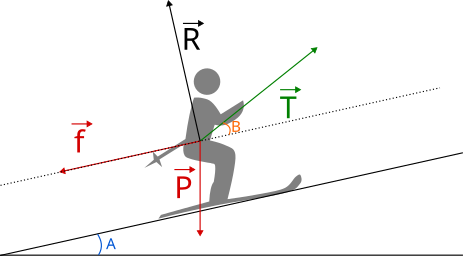
\includegraphics{fig28-1}
\subsubsection{b)\:Mouvement}
Le mouvement est rectiligne uniforme. D’après le principe d’inertie, les forces se compensent.
\subsubsection{b)\:Somme\:du\:Travail\:des\:forces}
Donc, la somme du travail des forces est nulle.
\subsection{2)\:Forces\:et\:travaux\:de\:forces}
$\overrightarrow{T}$ fournit un travail moteur, $\overrightarrow{R}$ fournit un travail nul (le vecteur R est perpendiculaire au déplacement, et $\cos (90) = 0$) , $\overrightarrow{f}$ et $\overrightarrow{P}$ fournissent un travail résistant.
\subsection{3)\:Trouver\:f}
\subsubsection{a)Différence\:d'altitude}

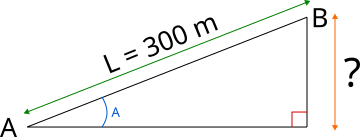
\includegraphics{fig28-2}

On modélise la situation par un triangle et on applique une propriété de trigonométrie. On note A le bas de la piste et B le sommet. Donc $$\sin(\alpha) = \frac{Oppose}{Hypothénuse} = \frac{Z_B - Z_A}{L} \Leftrightarrow Z_B - Z_A = L \times \sin(\alpha)$$

APP.N : $Z_B - Z_A = 300 \times \sin(22) = 11 \times 10^1 m$. On ne garde que 2 chiffres significatifs car la valeur la moins ``précise'', ici la mesure de l'angle, n'en possède que 2.
\subsubsection{b)Expression\:littérale\:du\:travail\:de\:chaque\:forces}
$W_{AB} (\overrightarrow{P}) = m \times g \times (Z_B - Z_A))$ On fait ``$Z_B - Z_A$``car on part du point A pour aller vers B dans cette situation.

$W_{AB} (\overrightarrow{R}) = R \times AB \times \cos(90) = R \times AB \times 0 = 0$

$W_{AB} (\overrightarrow{f}) = f \times AB \times \cos(180) = R \times AB \times (-1) = - f \times AB$

$W_{AB} (\overrightarrow{T}) = T \times AB \times \cos(B)$

APP.N :

$W_{AB} (\overrightarrow{P}) = m \times g \times (Z_B - Z_A)) = 85.5 \times 9.81 \times -11\times 10^1 = -9.2 \times 10^4\:$J

$W_{AB} (\overrightarrow{R}) = 0\:$J

$W_{AB} (\overrightarrow{f}) = - f \times AB$

$W_{AB} (\overrightarrow{T}) = T \times AB \times \cos(B) = 430 \times 11\times 10^1 \times \cos(30)= 4.0 \times 10^4\:$J

\subsubsection{c)Calcul\:de\:f}
La somme du travail des forces vaut 0, d'apres 1.b). Donc :
$$W_{AB} (\overrightarrow{R}) + W_{AB} (\overrightarrow{P}) + W_{AB} (\overrightarrow{T}) + W_{AB} (\overrightarrow{f}) = 0$$
$$W_{AB} (\overrightarrow{R}) + W_{AB} (\overrightarrow{P}) + W_{AB} (\overrightarrow{T}) = - W_{AB} (\overrightarrow{f})$$
$$W_{AB} (\overrightarrow{R}) + W_{AB} (\overrightarrow{P}) + W_{AB} (\overrightarrow{T}) = - (-f) \times AB$$
$$W_{AB} (\overrightarrow{R}) + W_{AB} (\overrightarrow{P}) + W_{AB} (\overrightarrow{T}) = f \times AB$$
$$\frac{W_{AB} (\overrightarrow{R}) + W_{AB} (\overrightarrow{P}) + W_{AB} (\overrightarrow{T})}{AB} = f$$

APP.N : $f = ||-47 \times 10^1|| = 47 \times 10^1$\: N
\end{document}
